\documentclass{ximera}

 

\usepackage{epsfig}

\graphicspath{
  {./}
  {figures/}
}

\usepackage{morewrites}
\makeatletter
\newcommand\subfile[1]{%
\renewcommand{\input}[1]{}%
\begingroup\skip@preamble\otherinput{#1}\endgroup\par\vspace{\topsep}
\let\input\otherinput}
\makeatother

\newcommand{\includeexercises}{\directlua{dofile("/home/jim/linearAlgebra/laode/exercises.lua")}}

%\newcounter{ccounter}
%\setcounter{ccounter}{1}
%\newcommand{\Chapter}[1]{\setcounter{chapter}{\arabic{ccounter}}\chapter{#1}\addtocounter{ccounter}{1}}

%\newcommand{\section}[1]{\section{#1}\setcounter{thm}{0}\setcounter{equation}{0}}

%\renewcommand{\theequation}{\arabic{chapter}.\arabic{section}.\arabic{equation}}
%\renewcommand{\thefigure}{\arabic{chapter}.\arabic{figure}}
%\renewcommand{\thetable}{\arabic{chapter}.\arabic{table}}

%\newcommand{\Sec}[2]{\section{#1}\markright{\arabic{ccounter}.\arabic{section}.#2}\setcounter{equation}{0}\setcounter{thm}{0}\setcounter{figure}{0}}

\newcommand{\Sec}[2]{\section{#1}}

\setcounter{secnumdepth}{2}
%\setcounter{secnumdepth}{1} 

%\newcounter{THM}
%\renewcommand{\theTHM}{\arabic{chapter}.\arabic{section}}

\newcommand{\trademark}{{R\!\!\!\!\!\bigcirc}}
%\newtheorem{exercise}{}

\newcommand{\dfield}{{\sf dfield9}}
\newcommand{\pplane}{{\sf pplane9}}

\newcommand{\EXER}{\section*{Exercises}}%\vspace*{0.2in}\hrule\small\setcounter{exercise}{0}}
\newcommand{\CEXER}{}%\vspace{0.08in}\begin{center}Computer Exercises\end{center}}
\newcommand{\TEXER}{} %\vspace{0.08in}\begin{center}Hand Exercises\end{center}}
\newcommand{\AEXER}{} %\vspace{0.08in}\begin{center}Hand Exercises\end{center}}

% BADBAD: \newcommand{\Bbb}{\bf}

\newcommand{\R}{\mbox{$\Bbb{R}$}}
\newcommand{\C}{\mbox{$\Bbb{C}$}}
\newcommand{\Z}{\mbox{$\Bbb{Z}$}}
\newcommand{\N}{\mbox{$\Bbb{N}$}}
\newcommand{\D}{\mbox{{\bf D}}}
\usepackage{amssymb}
%\newcommand{\qed}{\hfill\mbox{\raggedright$\square$} \vspace{1ex}}
%\newcommand{\proof}{\noindent {\bf Proof:} \hspace{0.1in}}

\newcommand{\setmin}{\;\mbox{--}\;}
\newcommand{\Matlab}{{M\small{AT\-LAB}} }
\newcommand{\Matlabp}{{M\small{AT\-LAB}}}
\newcommand{\computer}{\Matlab Instructions}
\newcommand{\half}{\mbox{$\frac{1}{2}$}}
\newcommand{\compose}{\raisebox{.15ex}{\mbox{{\scriptsize$\circ$}}}}
\newcommand{\AND}{\quad\mbox{and}\quad}
\newcommand{\vect}[2]{\left(\begin{array}{c} #1_1 \\ \vdots \\
 #1_{#2}\end{array}\right)}
\newcommand{\mattwo}[4]{\left(\begin{array}{rr} #1 & #2\\ #3
&#4\end{array}\right)}
\newcommand{\mattwoc}[4]{\left(\begin{array}{cc} #1 & #2\\ #3
&#4\end{array}\right)}
\newcommand{\vectwo}[2]{\left(\begin{array}{r} #1 \\ #2\end{array}\right)}
\newcommand{\vectwoc}[2]{\left(\begin{array}{c} #1 \\ #2\end{array}\right)}

\newcommand{\ignore}[1]{}


\newcommand{\inv}{^{-1}}
\newcommand{\CC}{{\cal C}}
\newcommand{\CCone}{\CC^1}
\newcommand{\Span}{{\rm span}}
\newcommand{\rank}{{\rm rank}}
\newcommand{\trace}{{\rm tr}}
\newcommand{\RE}{{\rm Re}}
\newcommand{\IM}{{\rm Im}}
\newcommand{\nulls}{{\rm null\;space}}

\newcommand{\dps}{\displaystyle}
\newcommand{\arraystart}{\renewcommand{\arraystretch}{1.8}}
\newcommand{\arrayfinish}{\renewcommand{\arraystretch}{1.2}}
\newcommand{\Start}[1]{\vspace{0.08in}\noindent {\bf Section~\ref{#1}}}
\newcommand{\exer}[1]{\noindent {\bf \ref{#1}}}
\newcommand{\ans}{}
\newcommand{\matthree}[9]{\left(\begin{array}{rrr} #1 & #2 & #3 \\ #4 & #5 & #6
\\ #7 & #8 & #9\end{array}\right)}
\newcommand{\cvectwo}[2]{\left(\begin{array}{c} #1 \\ #2\end{array}\right)}
\newcommand{\cmatthree}[9]{\left(\begin{array}{ccc} #1 & #2 & #3 \\ #4 & #5 &
#6 \\ #7 & #8 & #9\end{array}\right)}
\newcommand{\vecthree}[3]{\left(\begin{array}{r} #1 \\ #2 \\
#3\end{array}\right)}
\newcommand{\cvecthree}[3]{\left(\begin{array}{c} #1 \\ #2 \\
#3\end{array}\right)}
\newcommand{\cmattwo}[4]{\left(\begin{array}{cc} #1 & #2\\ #3
&#4\end{array}\right)}

\newcommand{\Matrix}[1]{\ensuremath{\left(\begin{array}{rrrrrrrrrrrrrrrrrr} #1 \end{array}\right)}}

\newcommand{\Matrixc}[1]{\ensuremath{\left(\begin{array}{cccccccccccc} #1 \end{array}\right)}}



\renewcommand{\labelenumi}{\theenumi)}
\newenvironment{enumeratea}%
{\begingroup
 \renewcommand{\theenumi}{\alph{enumi}}
 \renewcommand{\labelenumi}{(\theenumi)}
 \begin{enumerate}}
 {\end{enumerate}\endgroup}



\newcounter{help}
\renewcommand{\thehelp}{\thesection.\arabic{equation}}

%\newenvironment{equation*}%
%{\renewcommand\endequation{\eqno (\theequation)* $$}%
%   \begin{equation}}%
%   {\end{equation}\renewcommand\endequation{\eqno \@eqnnum
%$$\global\@ignoretrue}}

%\input{psfig.tex}

\author{Martin Golubitsky and Michael Dellnitz}

%\newenvironment{matlabEquation}%
%{\renewcommand\endequation{\eqno (\theequation*) $$}%
%   \begin{equation}}%
%   {\end{equation}\renewcommand\endequation{\eqno \@eqnnum
% $$\global\@ignoretrue}}

\newcommand{\soln}{\textbf{Solution:} }
\newcommand{\exercap}[1]{\centerline{Figure~\ref{#1}}}
\newcommand{\exercaptwo}[1]{\centerline{Figure~\ref{#1}a\hspace{2.1in}
Figure~\ref{#1}b}}
\newcommand{\exercapthree}[1]{\centerline{Figure~\ref{#1}a\hspace{1.2in}
Figure~\ref{#1}b\hspace{1.2in}Figure~\ref{#1}c}}
\newcommand{\para}{\hspace{0.4in}}

\renewenvironment{solution}{\suppress}{\endsuppress}

\ifxake
\newenvironment{matlabEquation}{\begin{equation}}{\end{equation}}
\else
\newenvironment{matlabEquation}%
{\let\oldtheequation\theequation\renewcommand{\theequation}{\oldtheequation*}\begin{equation}}%
  {\end{equation}\let\theequation\oldtheequation}
\fi

\makeatother


\title{Hamiltonian Systems}

\begin{document}
\begin{abstract}
\end{abstract}
\maketitle


\label{sec:HamSys}
\index{Hamiltonian system}

In the previous sections we have considered solution techniques that
can be applied to {\em scalar\/} differential equations.  In this section 
we present {\em planar\/} ODEs of a specific structure for which 
--- similar to the case of exact differential equations, see 
Section~\ref{S:exact} --- solutions
can be identified as level curves of a certain function.

An autonomous\index{autonomous} planar system of differential equations 
\begin{equation}  \label{e:ham}
\begin{array}{rcl} 
\dot{x} & = & f(x,y) \\
\dot{y} & = & g(x,y) 
\end{array}
\end{equation}
is {\em Hamiltonian\/}\index{Hamiltonian system} if there exists a real-valued
function $H(x,y)$ such that 
\[
f(x,y) = \frac{\partial H}{\partial y}(x,y) \AND 
g(x,y) =-\frac{\partial H}{\partial x}(x,y).
\]
The function $H$ is called the {\em Hamiltonian\/}\index{Hamiltonian system}
of the system \Ref{e:ham}.
By the following result Hamiltonian systems can be solved in a way analogous 
to exact systems.

\begin{thm}
Every solution trajectory of the Hamiltonian system \Ref{e:ham} lies
on a level curve\index{level curve} of the associated Hamiltonian $H$.
\end{thm}

\begin{proof} 
Let $(x(t),y(t))$ be a solution trajectory of \Ref{e:ham}.  We need to 
verify that $H(x(t),y(t))$ is constant in $t$.  This is most easily 
accomplished by showing that 
\begin{equation} \label{e:dH=0}
\frac{d}{dt} H(x(t),y(t)) = 0.
\end{equation}
Evaluate the left hand side of \Ref{e:dH=0} by using the chain rule:
\begin{eqnarray*}
\frac{d}{dt} H(x(t),y(t)) & = & \frac{\partial H}{\partial x}\frac{dx}{dt}
+ \frac{\partial H}{\partial y} \frac{dy}{dt} \\
& = & -g\frac{dx}{dt} + f\frac{dy}{dt}, 
\end{eqnarray*}
where the last equality follows from the definition of the Hamiltonian.  
Using the fact that $(x(t),y(t))$ is a solution of \Ref{e:ham} leads to 
\[
 \frac{d}{dt} H(x(t),y(t)) = -gf+fg = 0,
\]
as desired.  \end{proof}

\subsection*{Potential Systems}
\index{potential!system}
The system of differential equations
\begin{equation}  \label{e:hamex}
\begin{array}{rcl} 
\dot{x} & = & y \\
\dot{y} & = & -V'(x) 
\end{array}
\end{equation}
is a Hamiltonian system for any {\em potential\/} function $V(x)$,
\index{potential!function}
where the Hamiltonian\index{Hamiltonian system} is
\[
H(x,y) = \frac{1}{2}y^2 + V(x).
\]
To verify this point, just check that 
\[
-\frac{\partial H}{\partial x} = -V'(x) \AND \frac{\partial H}{\partial y} = y.
\]

In particular, the linear center\index{center} is a 
Hamiltonian system\index{Hamiltonian system}; just take 
$V(x)=\frac{1}{2}x^2$ so that 
\[
H(x,y) = \frac{1}{2}(x^2+y^2).
\]
Note that the level curves of this Hamiltonian are just circles centered 
at the origin.  This observation provides a second verification that 
trajectories of this center lie on circles.

A more interesting example occurs if we take the potential function 
equal to 
\[
V(x) = \frac{1}{4}x^4 - \frac{1}{2}x^2.
\]
The corresponding Hamiltonian system is:
\begin{equation*}  \label{e:hamex1}
\begin{array}{rcl} 
\dot{x} & = & y \\
\dot{y} & = & x-x^3 
\end{array}
\end{equation*}%
since $V'(x)=x^3-x$.  It is easy to verify that \Ref{e:hamex1} has three 
equilibria at $(1,0)$, $(0,0)$, and $(-1,0)$.  

The Jacobian of \Ref{e:hamex} is
\[
J = \left(\begin{array}{cc}  0 & 1 \\ -V''(x) & 0 \end{array}\right).
\]
Thus equilibria of \Ref{e:hamex} are saddles\index{saddle} 
if $V''<0$ or centers if $V''>0$.
Indeed, this dichotomy is generally valid for Hamiltonian systems and 
Hamiltonian systems are {\em not\/} usually Morse-Smale.  For instance, in
\Ref{e:hamex1} 
\[
V''(x) = 3x^2-1
\]
and the origin is a saddle while the other two equilibria are centers. 

For planar Hamiltonian systems, it is always the case (this is a theorem
similar to the Hopf bifurcation theorem) that centers are surrounded by 
a continuous family of periodic 
trajectories\index{family of periodic solutions}.  Using 
{\sf pplane5}\index{\computer!pplane5} we can
compute the phase portrait\index{phase!portrait} for 
this potential system\index{potential!system} and verify the 
existence of continuous families of periodic trajectories.  The result 
is presented in Figure~\ref{F:hamex}.  Note the numerical evidence for 
the existence of two homoclinic trajectories\index{trajectory!homoclinic}.  
\begin{figure}[htb]
           \centerline{%
	   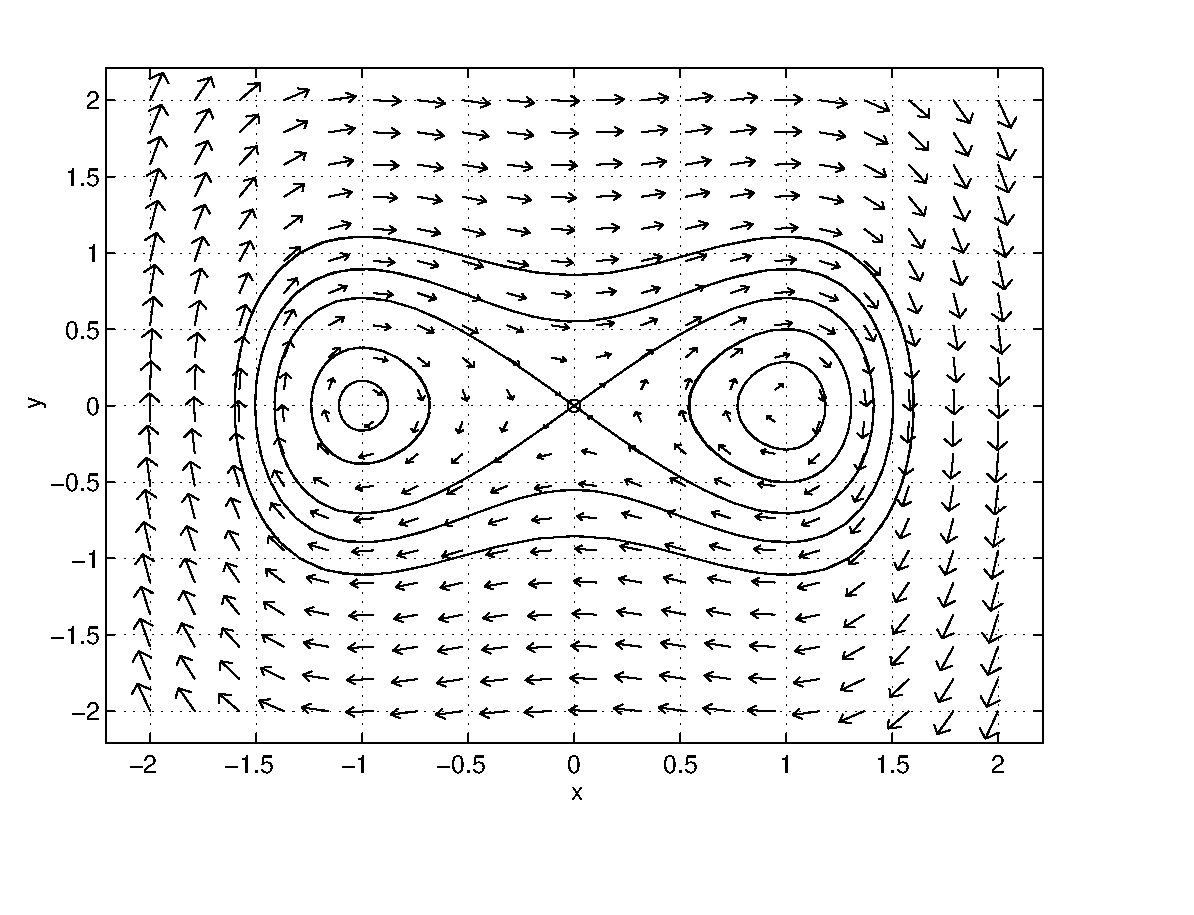
\psfig{file=figures/ham.eps,width=3.5in}}
           \caption{Phase portrait of \protect\Ref{e:hamex1}}
           \label{F:hamex}
\end{figure}

We remark that the system \Ref{e:hamex} is just the one obtained from the 
second order equation 
\begin{equation}  \label{e:V(x)}
\ddot{x} + V(x) = 0
\end{equation}
by the trick of setting $y=\dot{x}$ to obtain a planar system. 

\subsection*{Newton's Second Law and Potential Systems}
\index{potential!system}

There are several related interpretations of the potential $V$ in
\Ref{e:hamex} all based on Newton's second law of motion. 
\index{Newton's second law}  In particular, we can rewrite \Ref{e:V(x)} as 
\[
\ddot{x} =  -V(x)
\]
and interpret $-V$ as the force acting on a 
particle\index{particle motion} of unit mass\index{mass}.  In this 
interpretation it is assumed that the force just depends on the value of $x$. 

We consider three examples.
\begin{itemize}
\item[(a)] Suppose that $x$ is the position of a unit mass on a vertical 
line moving under the influence of gravity.  Then $V(x)=g$, where 
$g$ is the gravitational constant.
\item[(b)] Suppose that $x$ is the distance of a particle of unit mass from 
the sun.  The gravitational attraction of the sun is given by the inverse
square law. Assuming that the sun is at the origin, $V(x)= \frac{1}{x^2}$.
\item[(c)] Consider a pendulum\index{pendulum} 
with a unit mass attached to its end.  Assume, 
that the pendulum itself is idealized to have unit length and zero mass.  
The motion of an ideal pendulum is driven only by gravity. To derive the 
force acting on the pendulum, let $x$ be the angle that the pendulum makes 
with the vertical, as in Figure~\ref{F:pendulum}.  In that figure, the angle
$z=\frac{\pi}{2}-x$.  Then the force on the pendulum is $g\cos z=g\sin x$ 
and the pendulum equation is:
\begin{equation*} \label{e:pendulum}
\begin{array}{rcl} 
\dot{x} & = & y \\
\dot{y} & = & -g\sin x. 
\end{array}
\end{equation*}
\end{itemize}
\begin{figure}[htb]
           \centerline{%
	   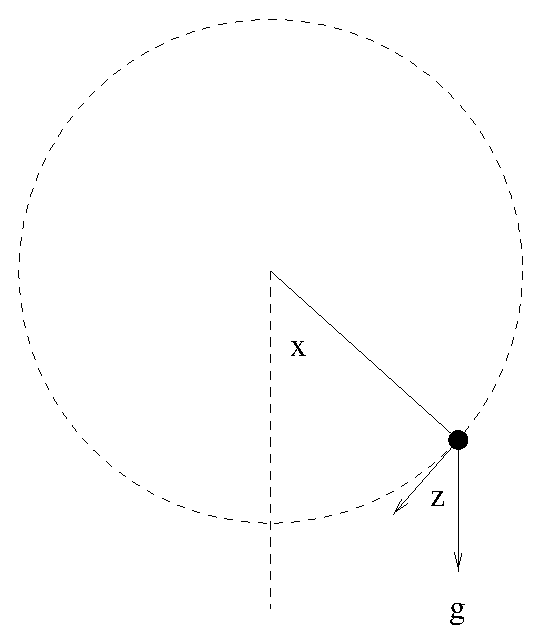
\psfig{file=figures/pendulum.eps,width=2.0in}}
           \caption{Pendulum geometry}
           \label{F:pendulum}
\end{figure}
The phase portrait for the pendulum equations is shown in Figure~\ref{F:ppen}.
\begin{figure}[htb]
           \centerline{%
	   \psfig{file=figures/ppen.eps,width=3.5in}}
           \caption{Phase portrait of the pendulum equation 
		\protect\Ref{e:pendulum}}
           \label{F:ppen}
\end{figure}


\subsubsection*{The Two Body Problem}

As a final example, consider the motion of two bodies of masses $m_1$ and 
$m_2$ under the influence of an attractive inverse square law of force.  Both 
bodies move in three dimensional space and therefore their motion would in 
principle be described by a system of three second order ODEs. However, by 
considering the motion inside an appropriate moving frame it is possible to 
neglect both the translational motion in space and the rotation of the two 
bodies around their common center of mass.  If this is done then the relative 
motion of the two bodies is described by the single second order equation
\begin{equation} \label{E:2body}
m\ddot x = -\frac{1}{x^2} + \frac{\ell^2}{mx^3}.
\end{equation}
Here $x(t)$ is the distance between the two bodies at time $t$,  $\ell$ is 
the (constant) {\em angular momentum\/} related to their rotational motion, 
and $m=m_1 m_2/(m_1 + m_2)$ is the {\em reduced mass}. 
We can rewrite \Ref{E:2body} in the form $\ddot{x}+V(x)=0$ where
\[
V(x) =  \frac{1}{mx^2} - \frac{\ell^2}{m^2x^3}.
\]
For two unit masses $m_1=m_2=1$ (that is, $m=1/2$) with angular momentum 
$\ell = 1$, we can rewrite the second order equation as the first order system 
\begin{equation*} \label{e:tbp}
\begin{array}{rcl}
\dot{x} & = & y \\
\dot{y} & = & -\frac{2}{x^2} + \frac{4}{x^3}.
\end{array}
\end{equation*}
The phase portrait of \Ref{e:tbp} is shown in Figure~\ref{fig:tbp}.  In 
physical space, the steady-state solution $(x,y)=(2,0)$ corresponds to a 
circular motion of the two bodies around their common center of mass and 
the periodic solutions correspond to motions on ellipsoids.

\begin{figure}[htb]
           \centerline{%
           \psfig{file=figures/tbp.eps,height=2.5in}}
           \caption{Phase portrait of the equation
                \protect\Ref{e:tbp}}
           \label{fig:tbp}
\end{figure}



\EXER

\TEXER

%\begin{exercise}
%Let $V(x) = x-x^3$.  Verify that the potential system \Ref{e:hamex} has
%three equilibria at the origin and at $(\pm 1,0)$.  Show that the origin 
%is a center and that the other equilibria are saddles.  Use {\sf pplane5}
%to find the phase portrait of this system.  How many heteroclinic 
%trajectories are there in this Hamiltonian system?
%\end{exercise}

\noindent In Exercises~\ref{c14.7.1} -- \ref{c14.7.4} write the system of 
differential equations corresponding to each of the given Hamiltonians. 
\begin{exercise} \label{c14.7.1}
$H(x,y) = x+3y+2$.
\end{exercise}
\begin{exercise} \label{c14.7.2}
$H(x,y) = y^3$.
\end{exercise}
\begin{exercise} \label{c14.7.3}
$H(x,y) = 1 + \sin x \cos y$.
\end{exercise}
\begin{exercise} \label{c14.7.4}
$H(x,y) = xy^2 - x + x\cos y$.
\end{exercise}

\noindent In Exercises~\ref{c14.7.5} -- \ref{c14.7.7} decide whether or not  
the given planar systems of differential equations is Hamiltonian:
\begin{exercise} \label{c14.7.5}
$\begin{array}{rcl}
\dot{x} & = & 0 \\
\dot{y} & = & -1.
\end{array}$
\end{exercise}
\begin{exercise} \label{c14.7.6}
$\begin{array}{rcl}
\dot{x} & = & x\\
\dot{y} & = & y.
\end{array}$
\end{exercise}
\begin{exercise} \label{c14.7.6a}
$\begin{array}{rcl}
\dot{x} & = & x - y^2\\
\dot{y} & = & -y - x^2.
\end{array}$
\end{exercise}
\begin{exercise} \label{c14.7.7}
$\begin{array}{rcl}
\dot{x} & = & x\cos y\\
\dot{y} & = & -\sin y.
\end{array}$
\end{exercise}

\begin{exercise} \label{c14.7.8}
Let $J$ be the Jacobian matrix of an equilibrium in a planar Hamiltonian 
system. Show that $\trace(J)=0$.  If $\det(J)\neq 0$, what are the possible
types for this equilibrium?
\end{exercise}

\begin{exercise} \label{c14.7.9}
Determine the equilibria in the pendulum equations \Ref{e:pendulum}.
Refer to the phase portrait of the ideal pendulum in Figure~\ref{F:ppen}
and describe in words the motion of the pendulum corresponding to a periodic 
solution surrounding one of the centers.  Describe the motion of the 
pendulum corresponding to the initial condition $(x(0),y(0))=(0,2)$.
\end{exercise}

\begin{exercise} \label{c14.7.10}
Consider the Hamiltonian  $H(x,y) = x^3 + x^2 - y^2$.  Show that the 
associated Hamiltonian system has a homoclinic trajectory.  {\bf Hint:} 
Consider the level curve $H(x,y)=0$.\index{homoclinic}
\end{exercise}

\begin{exercise} \label{c14.7.11} 
Consider the Hamiltonian  $H(x,y) = -\frac{1}{4}x^4 + \frac{1}{2}x^2 + y^2$.  
Show that the associated Hamiltonian system has saddle points at $(\pm 1,0)$ 
and heteroclinic trajectories connecting these saddle points.  {\bf Hint:} 
Consider the level curve $H(x,y) = \frac{1}{4}$.\index{heteroclinic}
\end{exercise}






 





\end{document}
